 vim: set spell spelllang=en tw=100 et sw=4 sts=4 foldmethod=marker foldmarker={{{,}}} :

\documentclass{beamer}

\usepackage{tikz}
\usepackage{xcolor}
\usepackage{complexity}
\usepackage{hyperref}
\usepackage{microtype}
\usepackage{amsmath}                   % \operatorname
\usepackage{amsfonts}                  % \mathcal
\usepackage{amssymb}                   % \nexists
\usepackage{gnuplot-lua-tikz}          % graphs

\usepackage[vlined]{algorithm2e} % algorithms
\usepackage{centernot}
\usepackage{mathtools}
\usepackage{listings}

\usetikzlibrary{shapes, arrows, shadows, calc, positioning, fit}
\usetikzlibrary{decorations.pathreplacing, decorations.pathmorphing, shapes.misc}
\usetikzlibrary{tikzmark}
\usetikzlibrary{knots}

\definecolor{uofguniversityblue}{rgb}{0, 0.219608, 0.396078}

\definecolor{uofgheather}{rgb}{0.356863, 0.32549, 0.490196}
\definecolor{uofgaquamarine}{rgb}{0.603922, 0.72549, 0.678431}
\definecolor{uofgslate}{rgb}{0.309804, 0.34902, 0.380392}
\definecolor{uofgrose}{rgb}{0.823529, 0.470588, 0.709804}
\definecolor{uofgmocha}{rgb}{0.709804, 0.564706, 0.47451}
\definecolor{uofgsandstone}{rgb}{0.321569, 0.278431, 0.231373}
\definecolor{uofgforest}{rgb}{0, 0.2, 0.129412}
\definecolor{uofglawn}{rgb}{0.517647, 0.741176, 0}
\definecolor{uofgcobalt}{rgb}{0, 0.615686, 0.92549}
\definecolor{uofgturquoise}{rgb}{0, 0.709804, 0.819608}
\definecolor{uofgsunshine}{rgb}{1.0, 0.862745, 0.211765}
\definecolor{uofgpumpkin}{rgb}{1.0, 0.72549, 0.282353}
\definecolor{uofgthistle}{rgb}{0.584314, 0.070588, 0.447059}
\definecolor{uofgrust}{rgb}{0.603922, 0.227451, 0.023529}
\definecolor{uofgburgundy}{rgb}{0.490196, 0.133333, 0.223529}
\definecolor{uofgpillarbox}{rgb}{0.701961, 0.047059, 0}
\definecolor{uofglavendar}{rgb}{0.356863, 0.301961, 0.580392}

%\tikzset{vertex/.style={draw, circle, inner sep=0pt, minimum size=0.5cm, font=\small\bfseries}}
%\tikzset{notvertex/.style={vertex, color=white, text=black}}
%\tikzset{plainvertex/.style={vertex}}
%\tikzset{vertexc1/.style={vertex, fill=uofgburgundy, text=white}}
%\tikzset{vertexc2/.style={vertex, fill=uofgsandstone, text=white}}
%\tikzset{vertexc3/.style={vertex, fill=uofgforest, text=white}}
%\tikzset{vertexc4/.style={vertex, fill=uofgheather, text=white}}
%\tikzset{edge/.style={color=black!50!white}}
%\tikzset{bedge/.style={ultra thick}}
%\tikzset{edged/.style={color=screengrey, dashed}}
%\tikzset{edgel3/.style={color=uofgrose, ultra thick}}

% {{{ theme things
\useoutertheme[footline=authortitle]{miniframes}
\useinnertheme{rectangles}

\setbeamerfont{block title}{size={}}
\setbeamerfont{title}{size=\large,series=\bfseries}
\setbeamerfont{section title}{size=\large,series=\mdseries}
\setbeamerfont{author}{size=\normalsize,series=\mdseries}
\setbeamercolor*{structure}{fg=uofguniversityblue}
\setbeamercolor*{palette primary}{use=structure,fg=black,bg=white}
\setbeamercolor*{palette secondary}{use=structure,fg=white,bg=uofgcobalt}
\setbeamercolor*{palette tertiary}{use=structure,fg=white,bg=uofguniversityblue}
\setbeamercolor*{palette quaternary}{fg=white,bg=black}

\setbeamercolor*{titlelike}{parent=palette primary}

\beamertemplatenavigationsymbolsempty

\setbeamertemplate{title page}
{
    \begin{tikzpicture}[remember picture, overlay]
        \node at (current page.north west) {
            \begin{tikzpicture}[remember picture, overlay]
                \fill [fill=uofguniversityblue, anchor=north west] (0, 0) rectangle (\paperwidth, -2.6cm);
            \end{tikzpicture}
        };

        \node (logo) [anchor=north east, shift={(-0.6cm,-0.6cm)}] at (current page.north east) {
            \includegraphics*[keepaspectratio=true,scale=0.7]{UoG_keyline.pdf}
        };

        \node [anchor=west, xshift=0.2cm] at (current page.west |- logo.west) {
            \begin{minipage}{0.65\paperwidth}\raggedright
                {\usebeamerfont{title}\usebeamercolor[white]{}\inserttitle}\\[0.1cm]
                {\usebeamerfont{author}\usebeamercolor[white]{}\insertauthor}
            \end{minipage}
        };
    \end{tikzpicture}
}

\setbeamertemplate{section page}
{
    \begin{centering}
        \begin{beamercolorbox}[sep=12pt,center]{part title}
            \usebeamerfont{section title}\insertsection\par
        \end{beamercolorbox}
    \end{centering}
}

\newcommand{\frameofframes}{/}
\newcommand{\setframeofframes}[1]{\renewcommand{\frameofframes}{#1}}

\makeatletter
\setbeamertemplate{footline}
{%
    \begin{beamercolorbox}[colsep=1.5pt]{upper separation line foot}
    \end{beamercolorbox}
    \begin{beamercolorbox}[ht=2.5ex,dp=1.125ex,%
        leftskip=.3cm,rightskip=.3cm plus1fil]{author in head/foot}%
        \leavevmode{\usebeamerfont{author in head/foot}\insertshortauthor}%
        \hfill%
        {\usebeamerfont{institute in head/foot}\usebeamercolor[fg]{institute in head/foot}\insertshortinstitute}%
    \end{beamercolorbox}%
    \begin{beamercolorbox}[ht=2.5ex,dp=1.125ex,%
        leftskip=.3cm,rightskip=.3cm plus1fil]{title in head/foot}%
        {\usebeamerfont{title in head/foot}\insertshorttitle}%
        \hfill%
        {\usebeamerfont{frame number}\usebeamercolor[fg]{frame number}\insertframenumber~\frameofframes~\inserttotalframenumber}
    \end{beamercolorbox}%
    \begin{beamercolorbox}[colsep=1.5pt]{lower separation line foot}
    \end{beamercolorbox}
}

% }}}

\title{Enumeration of (unique reduced alternating) knot diagrams}
\author[Ciaran McCreesh, Alice Miller, Patrick Prosser, Craig Reilly, James Trimble]{Ciaran McCreesh, Alice Miller, Patrick Prosser, \textbf{Craig Reilly}, James Trimble}

\begin{document}

{
    \usebackgroundtemplate{
        \tikz[overlay, remember picture]
        \node[at=(current page.south), anchor=south, inner sep=0pt]{\includegraphics*[keepaspectratio=true, width=\paperwidth]{background.jpg}};
    }
    \begin{frame}[plain,noframenumbering]
        \titlepage
    \end{frame}
}

\begin{frame}{What is a knot?}
    \begin{itemize}[<+->]
        \item A \emph{knot} is an embedding of the circle in $\mathbb{R}^3$.
        \item An intuitive way to think about this is to consider a knot as a knotted piece of string with the ends glued together.
    \end{itemize}
\end{frame}

\begin{frame}{Drawing knots on paper}
    \only<1> { 
        \begin{itemize}
            \item A function $f: \mathbb{R}^3 \rightarrow \mathbb{R}^2$ where $f(x, y, z) = f(x, y)$, is called a \emph{projection map}, and the image of a knot K under $f$ is called the \emph{projection} of K. 
            \item Such a projection is often refered to as the \emph{shadow} of K.
        \end{itemize}
    }
    \only<2> {
        \begin{itemize}
            \item Information regarding the orientation of arcs at crossings is given by leaving gaps in a knot's shadow..
        \end{itemize}
    }

    \begin{center}
    \only<3>{
    
\begin{tikzpicture}[every path/.style={uofgburgundy,ultra thick}, every node/.style={transform shape, knot crossing, inner sep=2.5pt}]
        \node[rotate=45] (tl) at (-1,1) {};
        \node[rotate=-45] (tr) at (1,1) {};
        \node (m) at (0,-1) {};
        \node (b) at (0,-2) {};
        \draw (b.center) .. controls (b.4 north west) and (m.4 south west) .. (m.center);
        \draw (b.center) .. controls (b.4 north east) and (m.4 south east) .. (m.center);
        \draw (m.center) .. controls (m.8 north west) and (tl.3 south west) .. (tl.center);
        \draw (m.center) .. controls (m.8 north east) and (tr.3 south east) .. (tr.center);
        \draw (tl.center) .. controls (tl.16 north east) and (tr.16 north west) .. (tr.center);
        \draw (b.center) .. controls (b.16 south east) and (tr.16 north east) .. (tr.center);
        \draw (b.center) .. controls (b.16 south west) and (tl.16 north west) .. (tl.center);
        \draw (tl.center) -- (tr.center);
    \end{tikzpicture}
    }
    \only<4>{
    
\begin{tikzpicture}[every path/.style={uofgburgundy,ultra thick}, every node/.style={transform shape, knot crossing, inner sep=2.5pt}]
        \node[rotate=45] (tl) at (-1,1) {};
        \node[rotate=-45] (tr) at (1,1) {};
        \node (m) at (0,-1) {};
        \node (b) at (0,-2) {};
        \draw (b) .. controls (b.4 north west) and (m.4 south west) .. (m.center);
        \draw (b.center) .. controls (b.4 north east) and (m.4 south east) .. (m);
        \draw (m) .. controls (m.8 north west) and (tl.3 south west) .. (tl.center);
        \draw (m.center) .. controls (m.8 north east) and (tr.3 south east) .. (tr);
        \draw (tl.center) .. controls (tl.16 north east) and (tr.16 north west) .. (tr);
        \draw (b) .. controls (b.16 south east) and (tr.16 north east) .. (tr.center);
        \draw (b.center) .. controls (b.16 south west) and (tl.16 north west) .. (tl);
        \draw (tl) -- (tr.center);
    \end{tikzpicture}
    }
\end{center}
\end{frame}

\begin{frame}{Representations of knots}
    \only<1>{
    \begin{itemize}
        \item Knot diagrams are really just 4-valent planar graphs.
            \begin{itemize}
                \item The vertices in the graph correspond to the crossings in the knot diagram.
                \item The arcs between vertices correspond to arcs between crossings in the knot diagram.
                \item The arcs are decorated with their orientation at their source and target crossings.
            \end{itemize}
        \item Other data structures familiar to computer scientists can be used, linked lists of crossings were popular in the 1950's.
    \end{itemize}
    }
    \only<2>
    {
    \begin{itemize}
        \item The representations used by topologists are typically also used for representing knots in a computer.
        \item Examples are Dowker-Thistlethwait codes (DT codes), \textbf{Gauss codes}, braid representatives, Conway notation, and many more.
    \end{itemize}
    }
\end{frame}

\begin{frame}{Representing knots with Gauss codes}
    \begin{columns}
        \begin{column}{0.65\textwidth}
            \begin{itemize}
            \item The strategy for representing a given knot (with $n$ crossings) by a Gauss code is as follows.
            \begin{enumerate}
                    \item Label the crossings with the numbers $1$ to $n$.
                    \item Pick a point on the knot.
                    \item Pick a direction and walk around the knot, writing out a list of the numbers you come to (with a negative sign indicating that a crossing was visited on an under strand).
            \end{enumerate}
            \end{itemize}
        \end{column}
        \begin{column}{0.25\textwidth}
            \begin{tikzpicture}[scale=0.7, every path/.style={uofgburgundy,ultra thick}, every node/.style={transform shape, knot crossing, inner sep=1.5pt}]
                \node[rotate=45] (tl) at (-1,1) {};
                \only<2-> \node[above left=0.2 of tl, color=uofgpillarbox]{1};
                \node[rotate=-45] (tr) at (1,1) {};
                \only<3-> \node[above right=0.2 of tr, color=uofgpillarbox]{2};
                \node (m) at (0,-1) {};
                \only<4-> \node[above=0.2 of m, color=uofgpillarbox]{3};
                \node (b) at (0,-2) {};
                \only<5-> \node[below=0.2 of b, color=uofgpillarbox]{4};
                
                \draw (b) .. controls (b.4 north west) and (m.4 south west) .. (m.center);
                \draw (b.center) .. controls (b.4 north east) and (m.4 south east) .. (m);
                \draw (m) .. controls (m.8 north west) and (tl.3 south west) .. (tl.center);
                \draw (m.center) .. controls (m.8 north east) and (tr.3 south east) .. (tr);
                \draw (tl.center) .. controls (tl.16 north east) and (tr.16 north west) .. (tr);
                \draw (b) .. controls (b.16 south east) and (tr.16 north east) .. (tr.center);
                \draw (b.center) .. controls (b.16 south west) and (tl.16 north west) .. (tl);
                \draw (tl) -- (tr.center);
            \end{tikzpicture}
        \end{column}
    \end{columns}
\end{frame}
% \begin{frame}{Two-Colouring a Triangle}
% 
%     \begin{columns}
%         \begin{column}{0.45\textwidth}
%             \begin{align*}
%                 & x_1 \in \{ 0, 1 \} \\
%                 & x_2 \in \{ 0, 1 \} \\
%                 & x_3 \in \{ 0, 1 \} \\
%                 & \mathrlap{\textit{alldifferent}( x_1, x_2, x_3 )} \\
%                 \\
%                 \\
%             \end{align*}
%         \end{column}
%                 \node [draw, ellipse] (C1) at (90:1.5) { $\{0,1\}$ };
%                 \node [draw, ellipse] (C2) at (210:1.5) { $\{0,1\}$ };
%                 \node [draw, ellipse] (C3) at (330:1.5) {  $\{0,1\}$  };
% 
%                 \node [anchor = south] (C) at (0, 0) { $\textit{alldifferent}$ };
% 
%                 \draw (C) to (C1);
%                 \draw (C) to (C2);
%                 \draw (C) to (C3);
%             \end{tikzpicture}
%         \end{column}
%     \end{columns}
% 
% \end{frame}
% 
% \begin{frame}{Decomposing ``All Different''}
% 
%     \begin{columns}
%         \begin{column}{0.45\textwidth}
%             \begin{align*}
%                 & x_1 \in \{ 0, 1 \} \\
%                 & x_2 \in \{ 0, 1 \} \\
%                 & x_3 \in \{ 0, 1 \} \\
%                 & x_1 \ne x_2 \\
%                 & x_1 \ne x_3 \\
%                 & x_2 \ne x_3 \\
%             \end{align*}
%         \end{column}
%         \begin{column}{0.45\textwidth}
%             \begin{tikzpicture}
%                 \node [draw, ellipse] (C1) at (90:1.5) { $\{0,1\}$ };
%                 \node [draw, ellipse] (C2) at (210:1.5) { $\{0,1\}$ };
%                 \node [draw, ellipse] (C3) at (330:1.5) {  $\{0,1\}$  };
% 
%                 \draw (C1) to node [xshift=-0.7em] { $\ne$ } (C2);
%                 \draw (C1) to node [xshift=0.7em] { $\ne$ } (C3);
%                 \draw (C2) to node [yshift=0.7em] { $\ne$ } (C3);
%             \end{tikzpicture}
%         \end{column}
%     \end{columns}
% 
% \end{frame}
% 
% \begin{frame}{What Does Propagation Do?}
% 
%     \begin{itemize}
%         \item Let's consider the constraint $x_1 \ne x_2$.
%             \begin{itemize}
%                 \item If $x_1 = 0$, we can give $x_2 = 1$, so that's OK.
%                 \item If $x_1 = 1$, we can give $x_2 = 0$, so that's OK.
%                 \item If $x_2 = 0$, we can give $x_1 = 1$, so that's OK.
%                 \item If $x_2 = 1$, we can give $x_1 = 0$, so that's OK.
%             \end{itemize}
%         \item Let's consider the constraint $x_1 \ne x_3$.
%             \begin{itemize}
%                 \item etc
%             \end{itemize}
%         \item Let's consider the constraint $x_2 \ne x_3$.
%             \begin{itemize}
%                 \item etc
%             \end{itemize}
%         \item So no values are deleted, and everything looks OK.
%         \item Actually, there's a more efficient algorithm: $\ne$ won't do anything unless one of
%             the variables only has one value. Some solvers won't trigger the constraint unless this
%             happens.
%     \end{itemize}
% 
% \end{frame}
% 
% \begin{frame}{What Would a Human Do?}
%     \begin{center}
%         ``Duh, obviously there's no solution! There \\ aren't enough numbers to go around.''
%     \end{center}
% 
%     \begin{itemize}
%         \item Unfortunately ``stare at it for a few seconds then write down the answer'' is not an algorithm.
% 
%         \item But if we don't decompose the constraint, we \emph{can} come up with a propagator
%             which can tell that there's no solution.
%     \end{itemize}
% \end{frame}
% 
% \begin{frame}{Matchings}
% 
%     \begin{columns}
%         \begin{column}{0.70\textwidth}
%             \begin{itemize}
%                 \item Draw a vertex on the left for each variable, and a vertex on the right for each value.
%                 \item Draw edges from each variable to each of its values.
%                 \item A \emph{maximum cardinality matching} is where you pick as many edges as
%                     possible, but each vertex can only be used at most once.
%                 \item We can find this in polynomial time (see Algorithmics II).
%                 \item There is a matching which covers each variable if and only if the constraint
%                     can be satisfied.
%             \end{itemize}
%         \end{column}
%         \begin{column}{0.28\textwidth}
%             \begin{tikzpicture}
%                 \node (X1) at (0, 2) { $x_1$ };
%                 \node (X2) at (0, 1) { $x_2$ };
%                 \node (X3) at (0, 0) { $x_3$ };
% 
%                 \node (V0) at (2, 2) { $0$ };
%                 \node (V1) at (2, 1) { $1$ };
%                 \node <3-> (V2) at (2, 0) { $2$ };
% 
%                 \draw <1, 3> [color=uofgsandstone!50] (X1) -- (V0);
%                 \draw <1, 3> [color=uofgsandstone!50] (X1) -- (V1);
%                 \draw <1, 3> [color=uofgsandstone!50] (X2) -- (V0);
%                 \draw <1, 3> [color=uofgsandstone!50] (X2) -- (V1);
%                 \draw <1, 3> [color=uofgsandstone!50] (X3) -- (V0);
%                 \draw <1, 3> [color=uofgsandstone!50] (X3) -- (V1);
%                 \draw <3> [color=uofgsandstone!50] (X2) -- (V2);
% 
%                 \draw <2> [color=uofgsandstone!50] (X1) -- (V1);
%                 \draw <2> [color=uofgsandstone!50] (X2) -- (V0);
%                 \draw <2> [color=uofgsandstone!50] (X3) -- (V0);
%                 \draw <2> [color=uofgsandstone!50] (X3) -- (V1);
%                 \draw <2> [ultra thick] (X1) -- (V0);
%                 \draw <2> [ultra thick] (X2) -- (V1);
% 
%                 \draw <4> [color=uofgsandstone!50] (X1) -- (V1);
%                 \draw <4> [color=uofgsandstone!50] (X2) -- (V0);
%                 \draw <4> [color=uofgsandstone!50] (X2) -- (V1);
%                 \draw <4> [color=uofgsandstone!50] (X3) -- (V0);
%                 \draw <4> [ultra thick] (X1) -- (V0);
%                 \draw <4> [ultra thick] (X3) -- (V1);
%                 \draw <4> [ultra thick] (X2) -- (V2);
%             \end{tikzpicture}
%         \end{column}
%     \end{columns}
% 
% \end{frame}
% 
% \begin{frame}{Sudoku}
% 
%     \centering
%     \includegraphics*[keepaspectratio=true,scale=0.18]{sudoku.png}
% 
% \end{frame}
% 
% \begin{frame}{How do Humans Solve Sudoku?}
%     \begin{center}\begin{tikzpicture}[scale=0.4]
%         \draw[thick, scale=3, color=uofgslate] (0, 0) grid (9, 1);
% 
%         \node <1>   [anchor=center] at (1.5, 1.5)  { 18 };
%         \node <2>   [anchor=center] at (1.5, 1.5)  { \textcolor{uofgcobalt}{1}8 };
%         \node <3>   [anchor=center] at (1.5, 1.5)  { \textcolor{uofgcobalt}{1} };
%         \node <4->  [anchor=center] at (1.5, 1.5)  { 1 };
% 
%         \node <1-4> [anchor=center] at (4.5, 1.5)  { 23 };
%         \node <5-6> [anchor=center] at (4.5, 1.5)  { \textcolor{uofgcobalt}{23} };
%         \node <7->  [anchor=center] at (4.5, 1.5)  { 23 };
% 
%         \node <1-4> [anchor=center] at (7.5, 1.5)  { 23 };
%         \node <5-6> [anchor=center] at (7.5, 1.5)  { \textcolor{uofgcobalt}{23} };
%         \node <7->  [anchor=center] at (7.5, 1.5)  { 23 };
% 
%         \node <1-5> [anchor=center] at (10.5, 1.5) { 245 };
%         \node <6>   [anchor=center] at (10.5, 1.5) { \textcolor{uofgpillarbox}{2}45 };
%         \node <7>   [anchor=center] at (10.5, 1.5) { 45 };
%         \node <8-9> [anchor=center] at (10.5, 1.5) { \textcolor{uofgcobalt}{45} };
%         \node <10-> [anchor=center] at (10.5, 1.5) { 45 };
% 
%         \node <1-7> [anchor=center] at (13.5, 1.5) { 456 };
%         \node <8-9>  [anchor=center] at (13.5, 1.5) { \textcolor{uofgcobalt}{456} };
%         \node <10-> [anchor=center] at (13.5, 1.5) { 456 };
% 
%         \node <1-7> [anchor=center] at (16.5, 1.5) { 456 };
%         \node <8-9> [anchor=center] at (16.5, 1.5) { \textcolor{uofgcobalt}{456} };
%         \node <10-> [anchor=center] at (16.5, 1.5) { 456 };
% 
%         \node <1-5> [anchor=center] at (19.5, 1.5) { 279 };
%         \node <6>   [anchor=center] at (19.5, 1.5) { \textcolor{uofgpillarbox}{2}79 };
%         \node <7->  [anchor=center] at (19.5, 1.5) { 79 };
% 
%         \node <1-5> [anchor=center] at (22.5, 1.5) { 378 };
%         \node <6>   [anchor=center] at (22.5, 1.5) { \textcolor{uofgpillarbox}{3}78 };
%         \node <7->  [anchor=center] at (22.5, 1.5) { 78 };
% 
%         \node <1-5> [anchor=center] at (25.5, 1.5) { 23589 };
%         \node <6>   [anchor=center] at (25.5, 1.5) { \textcolor{uofgpillarbox}{23}589 };
%         \node <7-8> [anchor=center] at (25.5, 1.5) { 589 };
%         \node <9>   [anchor=center] at (25.5, 1.5) { \textcolor{uofgpillarbox}{5}89 };
%         \node <10-> [anchor=center] at (25.5, 1.5) { 89 };
% 
%     \end{tikzpicture}\end{center}
% \end{frame}
% 
% \begin{frame}[fragile]{What Does Choco Do?}
%     \only<1> {
%         \lstinputlisting[language=Java, basicstyle=\scriptsize\ttfamily, keywordstyle=\color{uofgcobalt}]{code/OneRowSudoku-snippet.java}
%     }
% 
%     \only<2> {
%         \lstinputlisting[basicstyle=\scriptsize\ttfamily]{code/OneRowSudoku-output.txt}
% 
%         \begin{center}\begin{tikzpicture}[scale=0.4]
%             \draw[thick, scale=3, color=uofgslate] (0, 0) grid (9, 1);
% 
%             \node [anchor=center] at (1.5, 1.5)  { 1 };
%             \node [anchor=center] at (4.5, 1.5)  { 23 };
%             \node [anchor=center] at (7.5, 1.5)  { 23 };
%             \node [anchor=center] at (10.5, 1.5) { 45 };
%             \node [anchor=center] at (13.5, 1.5) { 456 };
%             \node [anchor=center] at (16.5, 1.5) { 456 };
%             \node [anchor=center] at (19.5, 1.5) { 79 };
%             \node [anchor=center] at (22.5, 1.5) { 78 };
%             \node [anchor=center] at (25.5, 1.5) { 89 };
% 
%         \end{tikzpicture}\end{center}
%     }
% 
%     \only<3> {
%         \lstinputlisting[language=Java, basicstyle=\scriptsize\ttfamily, keywordstyle=\color{uofgcobalt}]{code/OneRowSudoku-neq-snippet.java}
%     }
% 
%     \only<4> {
%         \lstinputlisting[basicstyle=\scriptsize\ttfamily]{code/OneRowSudoku-neq-output.txt}
%     }
% \end{frame}
% 
% \begin{frame}{Hall Sets}
%     \begin{itemize}
%         \item A \emph{Hall set} of size $n$ is a set of $n$ variables from an ``all different''
%             constraint, whose domains have $n$ values between them.
% 
%         \item If we can find a Hall set, we can safely remove these values from the domains of every
%             other variable involved in the constraint.
% 
%         \item If we do this for every Hall set, we delete every value that cannot appear in at least
%             one way of satisfying the constraint.
%     \end{itemize}
% \end{frame}
% 
% \begin{frame}{Only Occurs in One Place?}
% 
%     \begin{center}
%         ``But wait! We said that the value 1 only occurs \\
%         in one place. That doesn't sound like a Hall set!''
%     \end{center}
% 
%     \begin{itemize}
%         \item <2-> The ``only occurs in one place'' rule we used first is just a Hall set of size 8.
%     \end{itemize}
% \end{frame}
% 
% \begin{frame}{Is Choco Magic?}
% 
%     \only<1> {
%         \begin{itemize}
%             \item There are $2^n$ potential Hall sets, so considering them all is probably a bad
%                 idea. However, there is a polynomial algorithm.
% 
%             \item This algorithm isn't examinable, but here's an animation of roughly how it works,
%                 so you don't have to believe it's magic any more.
%         \end{itemize}
%     }
% 
%     \only <2-12> {
%         \begin{tikzpicture}[remember picture, overlay]
%             \node (logo) [anchor=north east, shift={(-0.4cm,-0.8cm)}] at (current page.north east) {
%                 \begin{tikzpicture}[scale=0.25, font=\tiny]
%                     \draw[thick, scale=3, color=uofgslate] (0, 0) grid (9, 1);
%                     \node <2-11> [anchor=center] at (1.5, 1.5)  { 18 };
%                     \node <2-11> [anchor=center] at (4.5, 1.5)  { 23 };
%                     \node <2-11> [anchor=center] at (7.5, 1.5)  { 23 };
%                     \node <2-11> [anchor=center] at (10.5, 1.5) { 245 };
%                     \node <2-11> [anchor=center] at (13.5, 1.5) { 456 };
%                     \node <2-11> [anchor=center] at (16.5, 1.5) { 456 };
%                     \node <2-11> [anchor=center] at (19.5, 1.5) { 279 };
%                     \node <2-11> [anchor=center] at (22.5, 1.5) { 378 };
%                     \node <2-11> [anchor=center] at (25.5, 1.5) { 23589 };
% 
%                     \node <12> [anchor=center] at (1.5, 1.5)  { \textcolor{uofgcobalt}{1}\textcolor{uofgpillarbox}{8} };
%                     \node <12> [anchor=center] at (4.5, 1.5)  { 23 };
%                     \node <12> [anchor=center] at (7.5, 1.5)  { 23 };
%                     \node <12> [anchor=center] at (10.5, 1.5) { \textcolor{uofgpillarbox}{2}45 };
%                     \node <12> [anchor=center] at (13.5, 1.5) { 456 };
%                     \node <12> [anchor=center] at (16.5, 1.5) { 456 };
%                     \node <12> [anchor=center] at (19.5, 1.5) { \textcolor{uofgpillarbox}{2}79 };
%                     \node <12> [anchor=center] at (22.5, 1.5) { \textcolor{uofgpillarbox}{3}78 };
%                     \node <12> [anchor=center] at (25.5, 1.5) { \textcolor{uofgpillarbox}{235}89 };
%                 \end{tikzpicture}
%             };
%         \end{tikzpicture}%
%         \centering
%         \begin{tikzpicture}[scale=0.75]
%             \path (-1, -0.6) rectangle (7, 8.6);
%             \node <3-> [inner sep = 1pt] (X1) at (0, 8) { $\mathit{row}[0]$ };
%             \node <3-> [inner sep = 1pt] (X2) at (0, 7) { $\mathit{row}[1]$ };
%             \node <3-> [inner sep = 1pt] (X3) at (0, 6) { $\mathit{row}[2]$ };
%             \node <3-> [inner sep = 1pt] (X4) at (0, 5) { $\mathit{row}[3]$ };
%             \node <3-> [inner sep = 1pt] (X5) at (0, 4) { $\mathit{row}[4]$ };
%             \node <3-> [inner sep = 1pt] (X6) at (0, 3) { $\mathit{row}[5]$ };
%             \node <3-> [inner sep = 1pt] (X7) at (0, 2) { $\mathit{row}[6]$ };
%             \node <3-> [inner sep = 1pt] (X8) at (0, 1) { $\mathit{row}[7]$ };
%             \node <3-> [inner sep = 1pt] (X9) at (0, 0) { $\mathit{row}[8]$ };
% 
%             \node <4-> [inner sep = 1pt] (V1) at (6, 8) { $1\vphantom{[]}$ };
%             \node <4-> [inner sep = 1pt] (V2) at (6, 7) { $2\vphantom{[]}$ };
%             \node <4-> [inner sep = 1pt] (V3) at (6, 6) { $3\vphantom{[]}$ };
%             \node <4-> [inner sep = 1pt] (V4) at (6, 5) { $4\vphantom{[]}$ };
%             \node <4-> [inner sep = 1pt] (V5) at (6, 4) { $5\vphantom{[]}$ };
%             \node <4-> [inner sep = 1pt] (V6) at (6, 3) { $6\vphantom{[]}$ };
%             \node <4-> [inner sep = 1pt] (V7) at (6, 2) { $7\vphantom{[]}$ };
%             \node <4-> [inner sep = 1pt] (V8) at (6, 1) { $8\vphantom{[]}$ };
%             \node <4-> [inner sep = 1pt] (V9) at (6, 0) { $9\vphantom{[]}$ };
% 
%             \draw <5> [thick, color=uofgsandstone!50] (X1.east) to [out=0, in=180] (V1.west);
%             \draw <5> [thick, color=uofgsandstone!50] (X1.east) to [out=0, in=180] (V8.west);
%             \draw <5> [thick, color=uofgsandstone!50] (X2.east) to [out=0, in=180] (V2.west);
%             \draw <5> [thick, color=uofgsandstone!50] (X2.east) to [out=0, in=180] (V3.west);
%             \draw <5> [thick, color=uofgsandstone!50] (X3.east) to [out=0, in=180] (V2.west);
%             \draw <5> [thick, color=uofgsandstone!50] (X3.east) to [out=0, in=180] (V3.west);
%             \draw <5> [thick, color=uofgsandstone!50] (X4.east) to [out=0, in=180] (V2.west);
%             \draw <5> [thick, color=uofgsandstone!50] (X4.east) to [out=0, in=180] (V4.west);
%             \draw <5> [thick, color=uofgsandstone!50] (X4.east) to [out=0, in=180] (V5.west);
%             \draw <5> [thick, color=uofgsandstone!50] (X5.east) to [out=0, in=180] (V4.west);
%             \draw <5> [thick, color=uofgsandstone!50] (X5.east) to [out=0, in=180] (V5.west);
%             \draw <5> [thick, color=uofgsandstone!50] (X5.east) to [out=0, in=180] (V6.west);
%             \draw <5> [thick, color=uofgsandstone!50] (X6.east) to [out=0, in=180] (V4.west);
%             \draw <5> [thick, color=uofgsandstone!50] (X6.east) to [out=0, in=180] (V5.west);
%             \draw <5> [thick, color=uofgsandstone!50] (X6.east) to [out=0, in=180] (V6.west);
%             \draw <5> [thick, color=uofgsandstone!50] (X7.east) to [out=0, in=180] (V2.west);
%             \draw <5> [thick, color=uofgsandstone!50] (X7.east) to [out=0, in=180] (V7.west);
%             \draw <5> [thick, color=uofgsandstone!50] (X7.east) to [out=0, in=180] (V9.west);
%             \draw <5> [thick, color=uofgsandstone!50] (X8.east) to [out=0, in=180] (V3.west);
%             \draw <5> [thick, color=uofgsandstone!50] (X8.east) to [out=0, in=180] (V7.west);
%             \draw <5> [thick, color=uofgsandstone!50] (X8.east) to [out=0, in=180] (V8.west);
%             \draw <5> [thick, color=uofgsandstone!50] (X9.east) to [out=0, in=180] (V2.west);
%             \draw <5> [thick, color=uofgsandstone!50] (X9.east) to [out=0, in=180] (V3.west);
%             \draw <5> [thick, color=uofgsandstone!50] (X9.east) to [out=0, in=180] (V5.west);
%             \draw <5> [thick, color=uofgsandstone!50] (X9.east) to [out=0, in=180] (V8.west);
%             \draw <5> [thick, color=uofgsandstone!50] (X9.east) to [out=0, in=180] (V9.west);
% 
%             \draw <6> [thick, color=uofgsandstone!50] (X1.east) to [out=0, in=180] (V8.west);
%             \draw <6> [thick, color=uofgsandstone!50] (X2.east) to [out=0, in=180] (V2.west);
%             \draw <6> [thick, color=uofgsandstone!50] (X3.east) to [out=0, in=180] (V3.west);
%             \draw <6> [thick, color=uofgsandstone!50] (X4.east) to [out=0, in=180] (V2.west);
%             \draw <6> [thick, color=uofgsandstone!50] (X4.east) to [out=0, in=180] (V5.west);
%             \draw <6> [thick, color=uofgsandstone!50] (X5.east) to [out=0, in=180] (V4.west);
%             \draw <6> [thick, color=uofgsandstone!50] (X5.east) to [out=0, in=180] (V5.west);
%             \draw <6> [thick, color=uofgsandstone!50] (X6.east) to [out=0, in=180] (V4.west);
%             \draw <6> [thick, color=uofgsandstone!50] (X6.east) to [out=0, in=180] (V6.west);
%             \draw <6> [thick, color=uofgsandstone!50] (X7.east) to [out=0, in=180] (V2.west);
%             \draw <6> [thick, color=uofgsandstone!50] (X7.east) to [out=0, in=180] (V9.west);
%             \draw <6> [thick, color=uofgsandstone!50] (X8.east) to [out=0, in=180] (V3.west);
%             \draw <6> [thick, color=uofgsandstone!50] (X8.east) to [out=0, in=180] (V7.west);
%             \draw <6> [thick, color=uofgsandstone!50] (X9.east) to [out=0, in=180] (V2.west);
%             \draw <6> [thick, color=uofgsandstone!50] (X9.east) to [out=0, in=180] (V3.west);
%             \draw <6> [thick, color=uofgsandstone!50] (X9.east) to [out=0, in=180] (V5.west);
%             \draw <6> [thick, color=uofgsandstone!50] (X9.east) to [out=0, in=180] (V8.west);
%             \draw <6> [thick] (X9.east) to [out=0, in=180] (V9.west);
%             \draw <6> [thick] (X1.east) to [out=0, in=180] (V1.west);
%             \draw <6> [thick] (X2.east) to [out=0, in=180] (V3.west);
%             \draw <6> [thick] (X3.east) to [out=0, in=180] (V2.west);
%             \draw <6> [thick] (X4.east) to [out=0, in=180] (V4.west);
%             \draw <6> [thick] (X5.east) to [out=0, in=180] (V6.west);
%             \draw <6> [thick] (X6.east) to [out=0, in=180] (V5.west);
%             \draw <6> [thick] (X7.east) to [out=0, in=180] (V7.west);
%             \draw <6> [thick] (X8.east) to [out=0, in=180] (V8.west);
% 
%             \draw <7-8> [thick, ->] ($(X1.east)!0.25!(X1.north east)$) to [out=0, in=180] ($(V8.west)!0.25!(V8.north west)$);
%             \draw <7-8> [thick, ->] ($(X2.east)!0.25!(X2.north east)$) to [out=0, in=180] ($(V2.west)!0.25!(V2.north west)$);
%             \draw <7-8> [thick, ->] ($(X3.east)!0.25!(X3.north east)$) to [out=0, in=180] ($(V3.west)!0.25!(V3.north west)$);
%             \draw <7-8> [thick, ->] ($(X4.east)!0.25!(X4.north east)$) to [out=0, in=180] ($(V2.west)!0.25!(V2.north west)$);
%             \draw <7-8> [thick, ->] ($(X4.east)!0.25!(X4.north east)$) to [out=0, in=180] ($(V5.west)!0.25!(V5.north west)$);
%             \draw <7-8> [thick, ->] ($(X5.east)!0.25!(X5.north east)$) to [out=0, in=180] ($(V4.west)!0.25!(V4.north west)$);
%             \draw <7-8> [thick, ->] ($(X5.east)!0.25!(X5.north east)$) to [out=0, in=180] ($(V5.west)!0.25!(V5.north west)$);
%             \draw <7-8> [thick, ->] ($(X6.east)!0.25!(X6.north east)$) to [out=0, in=180] ($(V4.west)!0.25!(V4.north west)$);
%             \draw <7-8> [thick, ->] ($(X6.east)!0.25!(X6.north east)$) to [out=0, in=180] ($(V6.west)!0.25!(V6.north west)$);
%             \draw <7-8> [thick, ->] ($(X7.east)!0.25!(X7.north east)$) to [out=0, in=180] ($(V2.west)!0.25!(V2.north west)$);
%             \draw <7-8> [thick, ->] ($(X7.east)!0.25!(X7.north east)$) to [out=0, in=180] ($(V9.west)!0.25!(V9.north west)$);
%             \draw <7-8> [thick, ->] ($(X8.east)!0.25!(X8.north east)$) to [out=0, in=180] ($(V3.west)!0.25!(V3.north west)$);
%             \draw <7-8> [thick, ->] ($(X8.east)!0.25!(X8.north east)$) to [out=0, in=180] ($(V7.west)!0.25!(V7.north west)$);
%             \draw <7-8> [thick, ->] ($(X9.east)!0.25!(X9.north east)$) to [out=0, in=180] ($(V2.west)!0.25!(V2.north west)$);
%             \draw <7-8> [thick, ->] ($(X9.east)!0.25!(X9.north east)$) to [out=0, in=180] ($(V3.west)!0.25!(V3.north west)$);
%             \draw <7-8> [thick, ->] ($(X9.east)!0.25!(X9.north east)$) to [out=0, in=180] ($(V5.west)!0.25!(V5.north west)$);
%             \draw <7-8> [thick, ->] ($(X9.east)!0.25!(X9.north east)$) to [out=0, in=180] ($(V8.west)!0.25!(V8.north west)$);
%             \draw <7-8> [thick, <-] ($(X9.east)!0.25!(X9.south east)$) to [out=0, in=180] ($(V9.west)!0.25!(V9.south west)$);
%             \draw <7-8> [thick, <-] ($(X1.east)!0.25!(X1.south east)$) to [out=0, in=180] ($(V1.west)!0.25!(V1.south west)$);
%             \draw <7-8> [thick, <-] ($(X2.east)!0.25!(X2.south east)$) to [out=0, in=180] ($(V3.west)!0.25!(V3.south west)$);
%             \draw <7-8> [thick, <-] ($(X3.east)!0.25!(X3.south east)$) to [out=0, in=180] ($(V2.west)!0.25!(V2.south west)$);
%             \draw <7-8> [thick, <-] ($(X4.east)!0.25!(X4.south east)$) to [out=0, in=180] ($(V4.west)!0.25!(V4.south west)$);
%             \draw <7-8> [thick, <-] ($(X5.east)!0.25!(X5.south east)$) to [out=0, in=180] ($(V6.west)!0.25!(V6.south west)$);
%             \draw <7-8> [thick, <-] ($(X6.east)!0.25!(X6.south east)$) to [out=0, in=180] ($(V5.west)!0.25!(V5.south west)$);
%             \draw <7-8> [thick, <-] ($(X7.east)!0.25!(X7.south east)$) to [out=0, in=180] ($(V7.west)!0.25!(V7.south west)$);
%             \draw <7-8> [thick, <-] ($(X8.east)!0.25!(X8.south east)$) to [out=0, in=180] ($(V8.west)!0.25!(V8.south west)$);
% 
%             \draw <9> [thick, ->, color=uofglawn!80!black] ($(X2.east)!0.25!(X2.north east)$) to [out=0, in=180] ($(V2.west)!0.25!(V2.north west)$);
%             \draw <9> [thick, ->, color=uofglawn!80!black] ($(X3.east)!0.25!(X3.north east)$) to [out=0, in=180] ($(V3.west)!0.25!(V3.north west)$);
%             \draw <9> [thick, <-, color=uofglawn!80!black] ($(X2.east)!0.25!(X2.south east)$) to [out=0, in=180] ($(V3.west)!0.25!(V3.south west)$);
%             \draw <9> [thick, <-, color=uofglawn!80!black] ($(X3.east)!0.25!(X3.south east)$) to [out=0, in=180] ($(V2.west)!0.25!(V2.south west)$);
%             \draw <9> [thick, ->, color=uofgturquoise!80!black] ($(X4.east)!0.25!(X4.north east)$) to [out=0, in=180] ($(V5.west)!0.25!(V5.north west)$);
%             \draw <9> [thick, ->, color=uofgturquoise!80!black] ($(X5.east)!0.25!(X5.north east)$) to [out=0, in=180] ($(V4.west)!0.25!(V4.north west)$);
%             \draw <9> [thick, ->, color=uofgturquoise!80!black] ($(X5.east)!0.25!(X5.north east)$) to [out=0, in=180] ($(V5.west)!0.25!(V5.north west)$);
%             \draw <9> [thick, ->, color=uofgturquoise!80!black] ($(X6.east)!0.25!(X6.north east)$) to [out=0, in=180] ($(V4.west)!0.25!(V4.north west)$);
%             \draw <9> [thick, ->, color=uofgturquoise!80!black] ($(X6.east)!0.25!(X6.north east)$) to [out=0, in=180] ($(V6.west)!0.25!(V6.north west)$);
%             \draw <9> [thick, <-, color=uofgturquoise!80!black] ($(X4.east)!0.25!(X4.south east)$) to [out=0, in=180] ($(V4.west)!0.25!(V4.south west)$);
%             \draw <9> [thick, <-, color=uofgturquoise!80!black] ($(X5.east)!0.25!(X5.south east)$) to [out=0, in=180] ($(V6.west)!0.25!(V6.south west)$);
%             \draw <9> [thick, <-, color=uofgturquoise!80!black] ($(X6.east)!0.25!(X6.south east)$) to [out=0, in=180] ($(V5.west)!0.25!(V5.south west)$);
%             \draw <9> [thick, ->, color=uofgpumpkin!80!black] ($(X7.east)!0.25!(X7.north east)$) to [out=0, in=180] ($(V9.west)!0.25!(V9.north west)$);
%             \draw <9> [thick, ->, color=uofgpumpkin!80!black] ($(X8.east)!0.25!(X8.north east)$) to [out=0, in=180] ($(V7.west)!0.25!(V7.north west)$);
%             \draw <9> [thick, ->, color=uofgpumpkin!80!black] ($(X9.east)!0.25!(X9.north east)$) to [out=0, in=180] ($(V8.west)!0.25!(V8.north west)$);
%             \draw <9> [thick, <-, color=uofgpumpkin!80!black] ($(X9.east)!0.25!(X9.south east)$) to [out=0, in=180] ($(V9.west)!0.25!(V9.south west)$);
%             \draw <9> [thick, <-, color=uofgpumpkin!80!black] ($(X7.east)!0.25!(X7.south east)$) to [out=0, in=180] ($(V7.west)!0.25!(V7.south west)$);
%             \draw <9> [thick, <-, color=uofgpumpkin!80!black] ($(X8.east)!0.25!(X8.south east)$) to [out=0, in=180] ($(V8.west)!0.25!(V8.south west)$);
%             \draw <11-> [thick, <-, color=uofgcobalt] ($(X1.east)!0.25!(X1.south east)$) to [out=0, in=180] ($(V1.west)!0.25!(V1.south west)$);
%             \draw <9-10>  [thick, <-] ($(X1.east)!0.25!(X1.south east)$) to [out=0, in=180] ($(V1.west)!0.25!(V1.south west)$);
%             \draw <9-10>  [thick, ->] ($(X4.east)!0.25!(X4.north east)$) to [out=0, in=180] ($(V2.west)!0.25!(V2.north west)$);
%             \draw <9-10>  [thick, ->] ($(X7.east)!0.25!(X7.north east)$) to [out=0, in=180] ($(V2.west)!0.25!(V2.north west)$);
%             \draw <9-10>  [thick, ->] ($(X8.east)!0.25!(X8.north east)$) to [out=0, in=180] ($(V3.west)!0.25!(V3.north west)$);
%             \draw <9-10>  [thick, ->] ($(X9.east)!0.25!(X9.north east)$) to [out=0, in=180] ($(V2.west)!0.25!(V2.north west)$);
%             \draw <9-10>  [thick, ->] ($(X9.east)!0.25!(X9.north east)$) to [out=0, in=180] ($(V3.west)!0.25!(V3.north west)$);
%             \draw <9-10>  [thick, ->] ($(X9.east)!0.25!(X9.north east)$) to [out=0, in=180] ($(V5.west)!0.25!(V5.north west)$);
%             \draw <9-10>  [thick, ->] ($(X1.east)!0.25!(X1.north east)$) to [out=0, in=180] ($(V8.west)!0.25!(V8.north west)$);
%             \draw <11->  [thick, ->, color=uofgpillarbox] ($(X4.east)!0.25!(X4.north east)$) to [out=0, in=180] ($(V2.west)!0.25!(V2.north west)$);
%             \draw <11->  [thick, ->, color=uofgpillarbox] ($(X7.east)!0.25!(X7.north east)$) to [out=0, in=180] ($(V2.west)!0.25!(V2.north west)$);
%             \draw <11->  [thick, ->, color=uofgpillarbox] ($(X8.east)!0.25!(X8.north east)$) to [out=0, in=180] ($(V3.west)!0.25!(V3.north west)$);
%             \draw <11->  [thick, ->, color=uofgpillarbox] ($(X9.east)!0.25!(X9.north east)$) to [out=0, in=180] ($(V2.west)!0.25!(V2.north west)$);
%             \draw <11->  [thick, ->, color=uofgpillarbox] ($(X9.east)!0.25!(X9.north east)$) to [out=0, in=180] ($(V3.west)!0.25!(V3.north west)$);
%             \draw <11->  [thick, ->, color=uofgpillarbox] ($(X9.east)!0.25!(X9.north east)$) to [out=0, in=180] ($(V5.west)!0.25!(V5.north west)$);
%             \draw <11->  [thick, ->, color=uofgpillarbox] ($(X1.east)!0.25!(X1.north east)$) to [out=0, in=180] ($(V8.west)!0.25!(V8.north west)$);
% 
%             \begin{pgfonlayer}{background}
%                 \node <8-9> [rounded corners, fit = (X1), fill=uofgthistle] {};
%                 \node <8-9> [rounded corners, fit = (V1), fill=uofglavendar] {};
%                 \node <8-9> [rounded corners, fit = (X2) (X3) (V2) (V3), fill=uofglawn] {};
%                 \node <8-9> [rounded corners, fit = (X4) (X5) (X6) (V4) (V5) (V6), fill=uofgcobalt] {};
%                 \node <8-9> [rounded corners, fit = (X7) (X8) (X9) (V7) (V8) (V9), fill=uofgpumpkin] {};
%             \end{pgfonlayer}
%         \end{tikzpicture}
%     }
% 
%     \only<13>{
%         \begin{itemize}
%             \item There's one more special condition that can happen, if we have more values than
%                 domains.
%         \end{itemize}
%     }
% \end{frame}
% 
% \begin{frame}[fragile]{A Sudoku Solver in Choco}
%     \only<1>{\lstinputlisting[basicstyle=\scriptsize\ttfamily]{code/herald20061222E.txt}}
%     \only<2>{\lstinputlisting[language=Java, basicstyle=\scriptsize\ttfamily, keywordstyle=\color{uofgcobalt}]{code/Sudoku-1-snippet.java}}
%     \only<3>{\lstinputlisting[language=Java, basicstyle=\scriptsize\ttfamily, keywordstyle=\color{uofgcobalt}]{code/Sudoku-2-snippet.java}}
%     \only<4>{\lstinputlisting[language=Java, basicstyle=\scriptsize\ttfamily, keywordstyle=\color{uofgcobalt}]{code/Sudoku-3-snippet.java}}
%     \only<5>{\lstinputlisting[language=Java, basicstyle=\scriptsize\ttfamily, keywordstyle=\color{uofgcobalt}]{code/Sudoku-4-snippet.java}}
%     \only<6-7>{
%         \lstinputlisting[language=Java, basicstyle=\scriptsize\ttfamily, keywordstyle=\color{uofgcobalt}]{code/Sudoku-5-snippet.java}
%         \begin{tikzpicture}[remember picture, overlay]
%             \node [anchor=north east, xshift=-0.5cm, yshift=-1cm] at (current page.north east) {
%                 \only<7>{\includegraphics*[keepaspectratio=true,scale=0.45]{eww.jpg}}
%             };
%         \end{tikzpicture}
%     }
%     \only<8>{\lstinputlisting[language=Java, basicstyle=\scriptsize\ttfamily, keywordstyle=\color{uofgcobalt}]{code/Sudoku-6-snippet.java}}
%     \only<9>{\lstinputlisting[language=Java, basicstyle=\scriptsize\ttfamily, keywordstyle=\color{uofgcobalt}]{code/Sudoku-7-snippet.java}}
% \end{frame}
% 
% \begin{frame}[fragile]{Incidentally, 2D arrays in Gecode are Much Nicer}
%     \lstinputlisting[language=C++, basicstyle=\scriptsize\ttfamily, keywordstyle=\color{uofgcobalt}]{code/GecodeSudoku-snippet.cc}
% \end{frame}
% 
% \begin{frame}{Some Experiments}
%     \only<1> {
%         \lstinputlisting[basicstyle=\scriptsize\ttfamily]{code/herald20061222E.txt}
%     }
%     \only<2-3> {
%         \begin{columns}
%             \begin{column}{0.45\textwidth}
%                 \lstinputlisting[basicstyle=\scriptsize\ttfamily]{code/herald20061222E-neq.txt}
%             \end{column}
%             \begin{column}{0.45\textwidth}
%                 \only<3>{
%                     \lstinputlisting[basicstyle=\scriptsize\ttfamily]{code/herald20061222E-alldiff.txt}
%                 }
%             \end{column}
%         \end{columns}
%     }
% 
%     \only<4> {
%         \lstinputlisting[basicstyle=\scriptsize\ttfamily]{code/herald20061222H.txt}
%     }
%     \only<5-6> {
%         \begin{columns}
%             \begin{column}{0.45\textwidth}
%                 \lstinputlisting[basicstyle=\scriptsize\ttfamily]{code/herald20061222H-neq.txt}
%             \end{column}
%             \begin{column}{0.45\textwidth}
%                 \only<6>{
%                     \lstinputlisting[basicstyle=\scriptsize\ttfamily]{code/herald20061222H-alldiff.txt}
%                 }
%             \end{column}
%         \end{columns}
%     }
% 
%     \only<7> {
%         \lstinputlisting[basicstyle=\scriptsize\ttfamily]{code/times20070107.txt}
%     }
%     \only<8-9> {
%         \begin{columns}
%             \begin{column}{0.45\textwidth}
%                 \lstinputlisting[basicstyle=\scriptsize\ttfamily]{code/times20070107-neq.txt}
%             \end{column}
%             \begin{column}{0.45\textwidth}
%                 \only<9>{
%                     \lstinputlisting[basicstyle=\scriptsize\ttfamily]{code/times20070107-alldiff.txt}
%                 }
%             \end{column}
%         \end{columns}
%     }
% 
%     \only<10> {
%         \centering
%         \includegraphics*[keepaspectratio=true,scale=0.24]{hardest.png}
%     }
%     \only<11-12> {
%         \begin{columns}
%             \begin{column}{0.45\textwidth}
%                 \lstinputlisting[basicstyle=\scriptsize\ttfamily]{code/hardest-neq.txt}
%             \end{column}
%             \begin{column}{0.45\textwidth}
%                 \only<12>{
%                     \lstinputlisting[basicstyle=\scriptsize\ttfamily]{code/hardest-alldiff.txt}
%                 }
%             \end{column}
%         \end{columns}
%     }
% 
%     \only<13> {
%         \scalebox{0.7}{
%             \begin{minipage}{2\paperwidth}
%                 \lstinputlisting[basicstyle=\fontsize{5pt}{6pt}\ttfamily]{code/huge.txt}
%         \end{minipage}}
%     }
% 
%     \only<14-15> {
%         \begin{columns}[t]
%             \begin{column}{0.45\textwidth}
%                 \lstinputlisting[basicstyle=\scriptsize\ttfamily]{code/huge-neq.txt}
%             \end{column}
%             \begin{column}{0.45\textwidth}
%                 \only<14> {
%                     \lstinputlisting[basicstyle=\scriptsize\ttfamily\color{white}]{code/huge-alldiff.txt}
%                 }
%                 \only<15> {
%                     \lstinputlisting[basicstyle=\scriptsize\ttfamily]{code/huge-alldiff.txt}
%                 }
%             \end{column}
%         \end{columns}
%     }
% \end{frame}
% 
% \begin{frame}{Do Global Constraints Always Help?}
%     \begin{itemize}
%         \item Sometimes globals make a spectacular difference.
% 
%         \item Sometimes global constraints end up not giving any more deletions than their
%             decompositions, and can take longer to propagate. Sometimes extra deletions don't help
%             anyway.
% 
%         \item Some global constraints cannot be \emph{decomposed}. Any global constraint can be
%             \emph{encoded} using binary constraints in a very unpleasant way involving polynomially
%             many extra variables, but AC on an encoding can be weaker than GAC.
% 
%             \begin{itemize}
%                 \item Difficult homework: $a + b = c$ using binary constraints.
%             \end{itemize}
% 
%         \item Using globals isn't a \emph{guaranteed} benefit, but they make the model easier to
%             read, and it's easier to translate from globals to decompositions and encodings than the
%             other way around.
% 
%             \begin{itemize}
%                 \item Really easy homework: detecting all-different is \NP-hard.
%             \end{itemize}
%     \end{itemize}
% \end{frame}
% 
% \begin{frame}{Some Other Interesting Global Constraints}
% 
%     \begin{itemize}
%         \item All different except 0.
%         \item Global cardinality.
%         \item At least, at most, among.
%         \item $n$ Value.
%         \item Regular.
%     \end{itemize}
% 
% \end{frame}
% 
% \begin{frame}{Are You Smarter than a Constraint Solver?}
%     \only<1> {
%         \begin{center}\begin{tikzpicture}[scale=0.4]
%             \draw[thick, scale=3, color=uofgslate] (0, 0) grid (3, 3);
%             \draw[thick, scale=3, color=uofgslate] (3, 0) grid (9, 1);
% 
%             \node[anchor=center] at (4.5, 1.5) { 34 };
%             \node[anchor=center] at (7.5, 1.5) { 35 };
%             \node[anchor=center] at (7.5, 4.5) { 45 };
%             \node[anchor=center] at (13.5, 1.5) { 345 };
% 
%         \end{tikzpicture}\end{center}
%     }
% 
%     \only<2> {
%         \begin{itemize}
%             \item Remember: propagation only considers \emph{one constraint at a time}, and the only
%                 communication between constraints is by deleting values.
% 
%             \item Automatically combining certain constraints is an active research topic.
%                 \begin{itemize}
%                     \item But getting ``the best possible'' filtering from two ``all different''
%                         constraints simultaneously is \NP-hard\ldots
%                 \end{itemize}
%         \end{itemize}
%     }
% \end{frame}
% 
% \begin{frame}{This is Not The Exam Question}
% 
%     What is a \emph{Hall set}, and why is it useful for propagation? Use the following model to
%     illustrate your answer:
%     \begin{align*}
%         & x_1 \in \{ 4, 5 \}   && x_2 \in \{ 1, 2, 3, 4 \}  && x_3 \in \{ 3, 4, 5 \} \\
%         & x_4 \in \{ 5, 6 \}   && x_5 \in \{ 3, 5 \} \\
%         & \mathrlap{\textit{alldifferent}( x_1, x_2, x_3, x_4, x_5 )}
%     \end{align*}
% 
%     Suppose our solver did not have an ``all different'' constraint. Show how to rewrite this model
%     using only binary constraints.  What effect would this have on propagation? \\[0.2cm]
% 
%     Aside from propagation, describe another benefit of global constraints.
% 
% \end{frame}
% 
% \begin{frame}[plain,noframenumbering]
%     \begin{tikzpicture}[remember picture, overlay]
%         \node at (current page.north west) {
%             \begin{tikzpicture}[remember picture, overlay]
%                 \fill [fill=uofguniversityblue, anchor=north west] (0, 0) rectangle (\paperwidth, -1.7cm);
%             \end{tikzpicture}
%         };
% 
%         \node (logo) [anchor=north east, shift={(-0.3cm,-0.2cm)}] at (current page.north east) {
%             \includegraphics*[keepaspectratio=true,scale=0.55]{UoG_keyline.pdf}
%         };
%     \end{tikzpicture}
% \end{frame}
% 
\end{document}


